\documentclass[11pt,a4paper]{article}
\usepackage[T1]{fontenc}
\usepackage[ngerman]{babel}
\usepackage{lmodern}
\usepackage[a4paper,margin=24mm,headheight=15pt]{geometry}
\usepackage{amsmath,amssymb,graphicx,booktabs,tabularx,longtable,array}
\usepackage{xcolor,microtype,fancyhdr}
\usepackage{hyperref}
\definecolor{ink}{HTML}{17334D}
\definecolor{fdm}{HTML}{2864A3}
\definecolor{bt}{HTML}{B02B80}
\hypersetup{colorlinks=true,linkcolor=ink,urlcolor=fdm,citecolor=bt,
 pdftitle={Finite Differenzen und Balanced Truncation: Fehler, Laufzeiten und Adaptivität},
 pdfauthor={Numerischer Arbeitsbericht zum Repository Model reduction balanced truncation}}
\graphicspath{{figures/}}
\pagestyle{fancy}\fancyhf{}
\fancyhead[L]{\small FDM und Balanced Truncation}
\fancyhead[R]{\small Numerischer Vergleich}
\fancyfoot[C]{\thepage}
\setlength{\parindent}{0pt}\setlength{\parskip}{5pt}
\setlength{\emergencystretch}{2em}
\renewcommand{\arraystretch}{1.18}
\newcommand{\R}{\mathbb{R}}
\newcommand{\norm}[1]{\left\lVert#1\right\rVert}
\newcommand{\Hinfty}{\mathcal{H}_\infty}
\newcommand{\fig}[3]{\begin{figure}[htbp]\centering\includegraphics[width=\linewidth]{#1}\caption{#2}\label{#3}\end{figure}}
\makeatletter\let\tableinput\@@input\makeatother
\newcommand{\BreakEven}{7.9}
\newcommand{\ReferenceGap}{3.2e-06}
\newcommand{\PDEFloor}{0.00159}


\begin{document}
\hypersetup{pageanchor=false}
\begin{titlepage}
\vspace*{14mm}
{\color{ink}\Huge\bfseries Finite Differenzen\par und Balanced Truncation\par}
\vspace{8mm}
{\Large Fehler, Laufzeiten und adaptive Verfahren\par}
\vspace{5mm}
{\large Ein reproduzierbarer Vergleich an der zweidimensionalen Wärmeleitung\par}
\vspace{12mm}
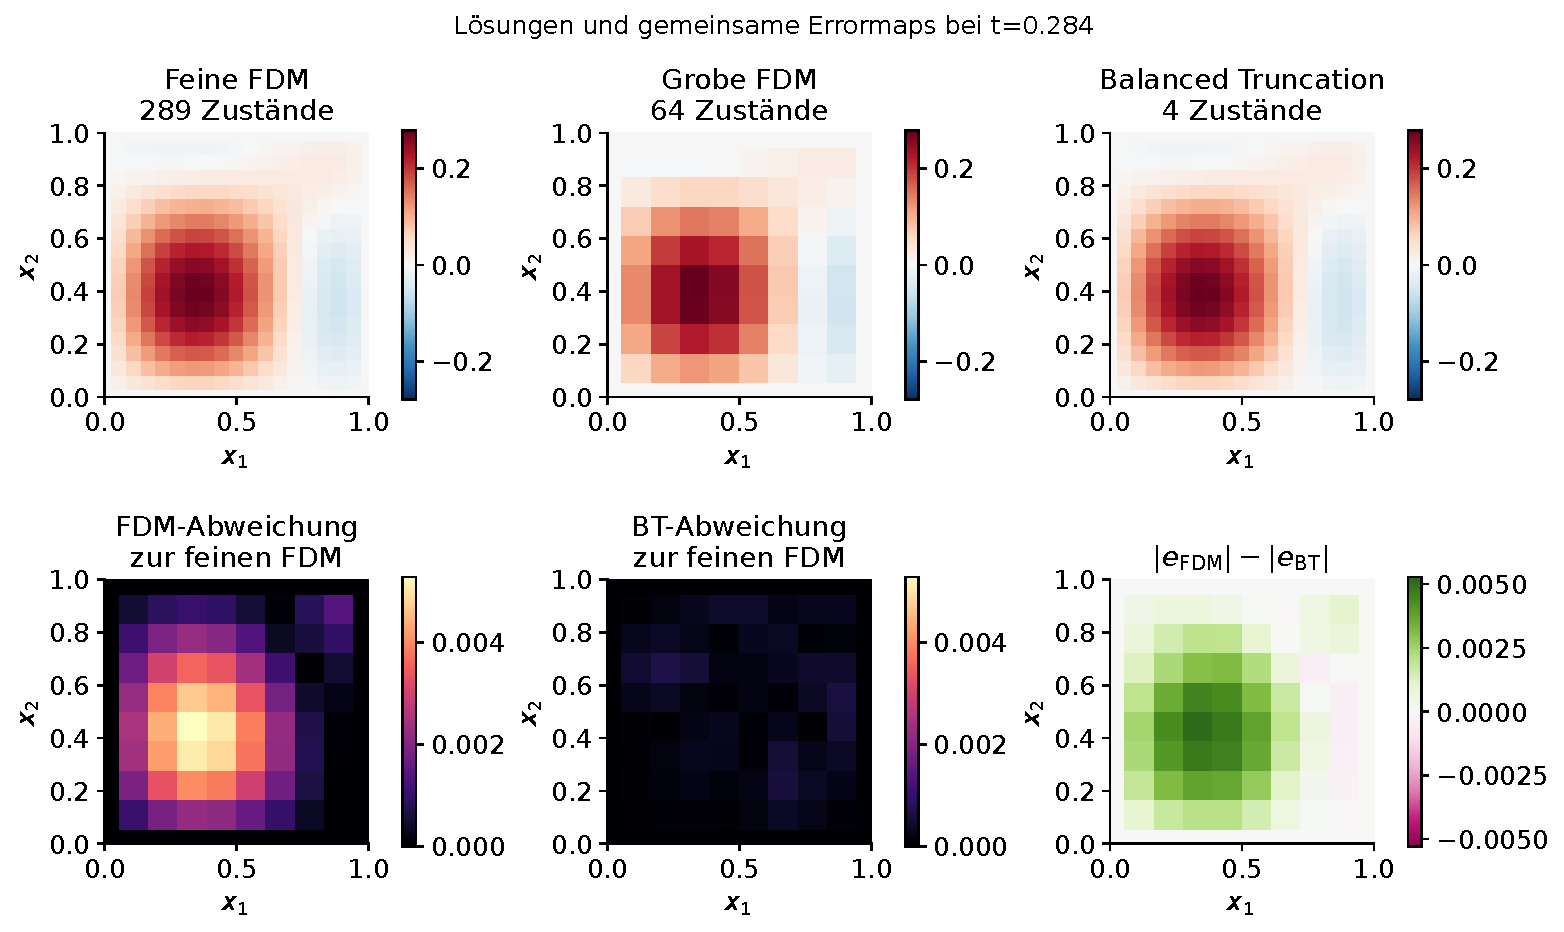
\includegraphics[width=\linewidth]{01_fields_errors.pdf}
\vfill
\textbf{Untersuchungsrahmen}\par
Aufgabenblatt 2, Model Reduction, TU Berlin, Wintersemester 2026/27.\par
Gemessene Daten vom 24.~November 2026. Python, NumPy und SciPy; doppelte Genauigkeit und ein BLAS-Thread.
\vspace{5mm}\par
\url{https://github.com/Darius-git-coder/Model_reduction_balanced_truncation}
\end{titlepage}
\pagenumbering{roman}
\hypersetup{pageanchor=true}

\section*{Ergebnisse auf einen Blick}
\addcontentsline{toc}{section}{Ergebnisse auf einen Blick}
Finite Differenzen (FDM) erzeugen aus einer partiellen Differentialgleichung ein räumliches Zustandsmodell. Balanced Truncation (BT) reduziert anschließend ein solches endliches Modell. Beide Methoden greifen damit auf unterschiedlichen Ebenen an und können kombiniert werden.

\begin{itemize}
\item Für die gegebene Anregung ist BT mit vier Zuständen deutlich kleiner als die grobe FDM mit 64 Zuständen. Der maximale Fehler zur gemeinsamen feinen FDM-Referenz ist in diesem Experiment etwa $1{,}04\cdot10^{-3}$ statt $5{,}35\cdot10^{-3}$; verglichen wird auf denselben 64 inneren Punkten.
\item Die BT-Konstruktion ist zunächst teuer. Bei wiederholten Simulationen mit unverändertem System amortisiert sie sich hier nach ungefähr \BreakEven\ Läufen gegenüber dem feinen FDM-Modell. Das ist ein aus gemessenen Komponenten abgeleiteter Schnittpunkt, keine allgemeine Konstante.
\item Ein größerer BT-Rang beseitigt den Raumfehler des Ausgangsmodells nicht. Im Rangexperiment nähert sich der Fehler zur unabhängigen PDE-Referenz einem Plateau von etwa \PDEFloor\ im punktweisen Maximum.
\item Die automatische Raum-/Rangwahl wird durch Richardson-Schätzer beziehungsweise die BT-Schranke gesteuert. Die unabhängige Referenz wird \emph{erst nach der Auswahl} zur Validierung verwendet. Ein Schätzer ist dabei nicht automatisch eine garantierte Fehlerschranke.
\item Adaptive Zeitschritte benötigen weniger akzeptierte Makroschritte, sind hier bei FDM aber trotzdem häufig langsamer: wechselnde Schrittweiten verursachen viele neue LU-Faktorisierungen. Laufzeit, Rechenarbeit und Schrittzahlen müssen gemeinsam betrachtet werden.
\end{itemize}

Der Bericht unterscheidet gemessene Fehler, asymptotische Schätzungen, theoretische Schranken und arithmetische Aufwandsmodelle. Es wird weder globale Optimalität der Adaptivität noch eine universelle Überlegenheit eines Verfahrens behauptet.
\tableofcontents
\clearpage
\pagenumbering{arabic}
\section{Problem, Physik und Vergleichsgegenstand}
Auf dem Einheitsquadrat $\Omega=(0,1)^2$ betrachten wir
\begin{align}
 \partial_t z(t,x)&=\Delta z(t,x)+b(x)u(t),\\
 b(x_1,x_2)&=\sin(3\pi x_1/2)\sin(4\pi x_2/3),\\
 z|_{\partial\Omega}&=0,\qquad z(0,x)=0.
\end{align}
Im Hauptversuch gilt $u(t)=10\sin(2\pi t)$ auf $[0,1]$. Das Produkt $b(x)u(t)$ ist örtlich und zeitlich vorzeichenbehaftet: Es beschreibt Wärmezufuhr und Wärmeentzug relativ zu einer Referenztemperatur. Eine periodische Antwort wird hier von außen erzwungen; sie ist kein Hinweis auf eine Wellengleichung. Ohne Anregung klingt die Lösung wegen des festgehaltenen Nullrandes gegen null ab. Die Erhaltung einer mittleren Temperatur würde andere Randbedingungen, etwa einen isolierten Rand ohne Quellen, voraussetzen.

Die beiden Ausgänge des Blattes sind
\begin{equation}
 y_1(t)=\int_\Omega z(t,x)\,dx,\qquad y_2(t)=z(t,\cdot).
\end{equation}
Eine Balancierung hängt von $B$ und $C$ ab: Ein für das Integral guter reduzierter Zustand muss nicht das gesamte räumliche Feld gleich gut wiedergeben. Die Feldvergleiche dieses Berichts verwenden deshalb $C_2=I$.

\begin{table}[htbp]\centering\small
\caption{Die wichtigsten strukturellen Unterschiede.}
\begin{tabularx}{\linewidth}{>{\raggedright\arraybackslash}p{30mm}>{\raggedright\arraybackslash}X>{\raggedright\arraybackslash}X}\toprule
Aspekt & Finite Differenzen & Balanced Truncation\\\midrule
Aufgabe & PDE räumlich diskretisieren & Vorhandenes LTI-System reduzieren\\
Zustände & Werte an Gitterpunkten & Globale gewichtete Zustandsrichtungen\\
Dimension & $n=d^2$, gekoppelt an $h$ & Ordnung $r$, gekoppelt an Hankel-Spektrum\\
Lokalität & Lokaler 5-Punkt-Stern; dünnbesetztes $A$ & Im Allgemeinen dichte reduzierte Matrizen\\
Eingang/Ausgang & Gitter meist unabhängig vom gewählten $C$ & Relevanz einer Richtung hängt von $B,C$ ab\\
Fehlerkontrolle & Konsistenzordnung, Schätzer, ggf. Residuenschranken & Globale Eingangs-Ausgangs-Schranke in $\Hinfty$\\
Erhaltung & Räumliche Struktur bleibt zugänglich & Stabilität unter Voraussetzungen; keine allgemeine Positivitäts- oder Erhaltungsgarantie\\
Änderung von $B,C$ & System/Operator anpassen & Erneute Balancierung kann nötig werden\\
Viele Simulationen & Große Zustandsdimension bleibt & Offline-Kosten können sich amortisieren\\\bottomrule
\end{tabularx}
\end{table}

\section{Finite Differenzen: vom Gitter zum LTI-System}
\subsection{Raumdiskretisierung und Speicherstruktur}
Mit $d$ inneren Punkten pro Richtung ist $h=1/(d+1)$. Der Parameter $d$ zählt Punkte; er ist kein Abstand. Die Randpunkte haben vorgegebene Werte und werden nicht als unabhängige Zustände gespeichert. Der klassische Stern lautet
\begin{equation}
 (\Delta_h z)_{ij}=\frac{z_{i+1,j}+z_{i-1,j}+z_{i,j+1}+z_{i,j-1}-4z_{ij}}{h^2}.
\end{equation}
Reihenweises Stapeln der inneren Werte ergibt $x\in\R^{d^2}$. Mit der eindimensionalen Differenzenmatrix $K=h^{-2}\operatorname{tridiag}(1,-2,1)$ entsteht
\begin{equation}
 A=I\otimes K+K\otimes I,\quad B_{ij}=b(ih,jh),\quad
 C_1=h^2\mathbf 1^\top,\quad C_2=I.
\end{equation}
Damit gilt $\dot x=Ax+Bu$ und $y=Cx$. Die Matrix hat auf dem regulären Gitter $5d^2-4d$ mathematisch von null verschiedene Einträge. Dünnbesetzte Formate speichern den Stern mit Aufwand $O(n)$; bei einer impliziten Lösung kann die LU-Zerlegung zusätzlich Füllung erzeugen.

Durch Taylorentwicklung erhält man bei ausreichender Glattheit
\begin{equation}
 \Delta_h z-\Delta z=\frac{h^2}{12}(\partial_{x_1}^4z+\partial_{x_2}^4z)+O(h^4).
\end{equation}
Das erklärt die zweite räumliche Konsistenzordnung. Randbehandlung, Regularität und Zeitdiskretisierung müssen ebenfalls stimmen, damit diese Ordnung im beobachteten Fehler erscheint. Eine ausführliche Einführung in räumliche Differenzenverfahren bietet beispielsweise \cite{kochmann}.

\subsection{Zeitintegration und Stabilität}
Der implizite Euler berechnet
\begin{equation}\label{eq:euler}
 (I-\Delta t A)x_{k+1}=x_k+\Delta t B u(t_{k+1}).
\end{equation}
Bei fester Schrittweite wird die linke Matrix einmal faktorisiert. Danach benötigt jeder Schritt nur noch einen linearen Lösevorgang. Auf glatten Lösungen ist der globale Zeitfehler erster Ordnung. Das führt unter passenden Voraussetzungen auf eine Gesamtform $O(h^2)+O(\Delta t)$, mit problemabhängigen Konstanten und Normen.

Die Eigenwerte des diskreten Laplaceoperators sind
\begin{equation}
 \lambda_{pq}=-\frac4{h^2}\left[\sin^2\!\frac{p\pi h}{2}+\sin^2\!\frac{q\pi h}{2}\right]<0.
\end{equation}
Der explizite Euler verlangt für den üblichen 2D-Stern insbesondere $\Delta t\le h^2/4$. Der implizite Euler ist für dieses Diffusionssystem ohne eine solche Stabilitätsbeschränkung einsetzbar. Große Schritte können trotzdem ungenau sein: Stabilität ersetzt keine Genauigkeitskontrolle.

\section{Balanced Truncation: Zustandsrichtungen auswählen}
\subsection{Gramians und ihre Bedeutung}
Für ein reelles asymptotisch stabiles LTI-System lösen wir
\begin{align}
 AP+PA^\top+BB^\top&=0,\\
 A^\top Q+QA+C^\top C&=0.
\end{align}
Es gilt
\begin{equation}
 P=\int_0^\infty e^{At}BB^\top e^{A^\top t}dt,\qquad
 Q=\int_0^\infty e^{A^\top t}C^\top Ce^{At}dt.
\end{equation}
Die symmetrischen positiv semidefiniten Gramians sind im Allgemeinen keine orthogonalen Projektoren. Bei erreichbaren Zuständen beschreibt $x^\top P^{-1}x$ die minimale Eingangsenergie zum Erreichen von $x$; $x^\top Qx$ ist die Ausgangsenergie der freien Antwort aus $x$ \cite{energy}. Eine Richtung kann stark anregbar, aber am Ausgang praktisch unsichtbar sein. Ihre Bedeutung für den gewählten Eingangs-Ausgangs-Kanal bleibt dann klein.

\subsection{Die fünf Schritte mit eindeutiger Konvention}
Wir verwenden $x_{\rm bal}=Tx$ und $x\approx\widetilde T x_{\rm bal}$. Ein hochgestelltes $\top$ bedeutet Transposition; es ist nicht die Transformationsmatrix $T$.
\begin{enumerate}
\item Löse die beiden Lyapunov-Gleichungen für $P,Q$.
\item Bilde Faktoren $P\approx RR^\top$, $Q\approx LL^\top$. Die bereitgestellte Routine \texttt{lrcf} erlaubt rechteckige Faktoren bei numerisch niedrigem Rang.
\item Berechne $L^\top R=U\Sigma V^\top$, mit absteigenden positiven Singulärwerten $\sigma_k$.
\item Setze
\begin{equation}
 T=\Sigma^{-1/2}U^\top L^\top,\qquad
 \widetilde T=RV\Sigma^{-1/2},\qquad T\widetilde T=I.
\end{equation}
\item Bilde $A_b=TA\widetilde T$, $B_b=TB$, $C_b=C\widetilde T$ und schneide auf die ersten $r$ Zustände zurück:
\begin{equation}
 A_b=\begin{pmatrix}A_{11}&A_{12}\\A_{21}&A_{22}\end{pmatrix},\quad
 B_b=\begin{pmatrix}B_1\\B_2\end{pmatrix},\quad C_b=(C_1\ C_2),\quad
 (A_r,B_r,C_r)=(A_{11},B_1,C_1).
\end{equation}
\end{enumerate}
Die blockweisen Bezeichnungen $C_1,C_2$ in dieser letzten Formel sind Blöcke der balancierten Ausgangsmatrix und nicht die beiden Beobachtungsvarianten des Aufgabenblattes.

In einer exakten minimalen balancierten Realisierung gilt $P_b=Q_b=\Sigma$. Die Diagonaleinträge müssen nicht gleich sein. Die Hankel-Singulärwerte erfüllen $\sigma_k=\sqrt{\lambda_k(PQ)}$. Die Vorschrift ist eine Projektion auf relevante globale Richtungen \cite{benner2023}. Bei rechteckigen Abbildungen ist $\widetilde T$ keine gewöhnliche Inverse; $\widetilde TT$ ist im Allgemeinen auch keine orthogonale Projektion.

\fig{10_global_directions.pdf}{Die ersten vier rekonstruierten BT-Richtungen für vollständige Zustandsbeobachtung. Jede Richtung erstreckt sich über das ganze Gebiet. Pro Teilbild wird eine eigene symmetrische Farbskala verwendet; daraus darf keine Gleichheit ihrer Bedeutung abgelesen werden.}{fig:modes}

\subsection{Was erhalten bleibt und was nicht}
Bei stabilem minimalem Ausgangssystem und einer zulässigen Trennung des Hankel-Spektrums, insbesondere $\sigma_r>\sigma_{r+1}$, bleibt die reduzierte Realisierung asymptotisch stabil \cite{lall}. Gruppen gleicher Singulärwerte sollten nicht willkürlich geteilt werden. Standard-BT garantiert im Allgemeinen weder Positivität noch ein diskretes Maximumprinzip noch physikalische Interpretierbarkeit jeder reduzierten Koordinate. Die übliche Fehlerschranke setzt Nullanfangswerte voraus. Für andere Anfangswerte oder veränderte Parameter sind zusätzliche Überlegungen nötig.

\section{Fehler, Referenzen und belastbare Aussagen}
\subsection{Drei verschiedene Fehlerquellen}
Räumliche Diskretisierung, Zeitintegration und Modellreduktion müssen getrennt werden. Schematisch gilt in einer gemeinsamen Norm und mit konsistenter Rekonstruktion $\mathcal I_h$
\begin{align}
 \norm{z-\mathcal I_h C_r x_r^{\Delta t}}
 &\le \underbrace{\norm{z-\mathcal I_h x_h}}_{\text{Raumfehler}}
 +\underbrace{\norm{\mathcal I_h(x_h-C_rx_r)}}_{\text{Reduktionsfehler}}\\
 &\quad+\underbrace{\norm{\mathcal I_h C_r(x_r-x_r^{\Delta t})}}_{\text{Zeitfehler}}.
\end{align}
Ein schrumpfender Reduktionsfehler allein beweist keine verbesserte PDE-Approximation. Verschiedene Fehler können sich in Einzelversuchen teilweise aufheben; monotone Punktfehler sind bei wachsendem $r$ nicht garantiert.

\subsection{Die BT-Schranke und ihre Reichweite}
Für $G(s)=C(sI-A)^{-1}B$ und den BT-Approximanten gilt im idealen exakten Rahmen
\begin{equation}\label{eq:btbound}
 \sigma_{r+1}\le\norm{G-G_r}_{\Hinfty}\le 2\sum_{k=r+1}^{n}\sigma_k.
\end{equation}
Die obere Schranke begrenzt die Verstärkung des Reduktionsfehlers über alle Frequenzen. Für Nullanfangswerte folgt
\begin{equation}
 \norm{y-y_r}_{L^2}\le 2\sum_{k>r}\sigma_k\,\norm{u}_{L^2}.
\end{equation}
Auf $[0,1]$ kann der Eingang danach mit null fortgesetzt werden; die kausale Antwort im Messfenster bleibt unverändert. Die Energieaussage gilt dann auch eingeschränkt auf dieses Fenster. Sie ist keine unmittelbare punktweise Schranke für jede Errormap \cite{lall,lower}.

Die Experimente verwenden numerisch komprimierte Gramians mit Toleranz $10^{-14}$. Die dargestellte Restsumme ist deshalb eine numerische Version der idealen Schranke; ein zusätzliches zertifiziertes Fehlerbudget für die Gramian-Kompression wird hier nicht konstruiert. Abgetastete Frequenzmaxima sind ebenfalls keine Beweise für das kontinuierliche Supremum. Die Stichprobe enthält null und 1\,000 logarithmische positive Frequenzen zwischen $10^{-5}$ und $10^5$; bei reellen Systemen ist die negative Seite konjugiert symmetrisch.

\subsection{Die im Bericht verwendeten Normen}
Die ersten Errormaps vergleichen grobe FDM und BT mit derselben feinen FDM-Lösung an den 64 groben inneren Punkten. Dort ist keine räumliche Interpolation nötig. Die Aussage betrifft die Diskretisierung des Blattes, nicht die exakte PDE.

Für den adaptiven Raum-/Rangvergleich verwenden wir dagegen ein festes Prüfgitter mit $19\times19$ Punkten einschließlich Rand und 101 Zeitpunkten. Bewertet wird die quadraturbasierte Energienorm
\begin{equation}\label{eq:energy}
 E(v)=\left(\operatorname{trapz}_{t\in[0,1]}\frac1{18^2}\sum_{i,j}|v_{ij}(t)|^2\right)^{1/2}.
\end{equation}
Gitterlösungen werden dazu bilinear auf dieselben Prüfpunkte übertragen. Zusätzlich werden punktweise Maxima angegeben. Fehler zwischen Prüfpunkten werden dadurch nicht zertifiziert. Der reine Zeitvergleich verwendet nochmals einen anderen, ausdrücklich so bezeichneten Fehler: Abweichung von der zeitlich exakten Lösung \emph{desselben} semidiskreten Modells.

\clearpage
\section{Versuchsaufbau und unabhängige Referenz}
\subsection{Reproduzierbare Messbedingungen}
Alle Zahlen wurden lokal mit Python 3.11.5, NumPy 1.26.4, SciPy 1.13.1 und OpenBLAS 0.3.21 auf einer x86\_64-Umgebung gemessen. Die BLAS-Bibliothek verwendet genau einen Thread; ihre gemeldete Kernelarchitektur ist Haswell. Das ist eine Softwareangabe und kein vollständiges Hardwareinventar. Absolute Zeiten hängen von Rechner, Auslastung und Bibliotheken ab.

Ein Aufwärmlauf wird verworfen. Für Online- und Zeitintegrationsmessungen wird der Median aus fünf Wiederholungen verwendet, für die kostspieligere Balancierung und adaptive Modellauswahl aus drei Wiederholungen. Quartile stehen in den CSV-Dateien. Aufbau, Faktorisierung, eigentliche Simulation und Feldrekonstruktion werden getrennt erfasst. Plotten, PDF-Erzeugung und Dateischreiben liegen außerhalb der gemessenen Abschnitte.

Die regulären Versuche verwenden $t_f=1$, 1\,000 feste Euler-Schritte und Nullanfangswerte. Für das Ausgangsmodell gilt $d=17$, $n=289$. Das grobe Modell besitzt $d=8$, $n=64$; das BT-Modell typischerweise $r=4$. Unterschiedliche Zustandszahlen sind ausdrücklich sichtbar. Das ist kein Vergleich bei identischem Rechenbudget. Ein Vergleich bei gleicher Fehlerqualität ist aussagekräftiger als die bloße Forderung gleicher Dimensionen.

\subsection{Sinusreihe statt nur eines feineren Gitters}
Da Randbedingungen und Geometrie einfach sind, lässt sich eine unabhängige Referenz aus Eigenfunktionen der kontinuierlichen Wärmegleichung gewinnen:
\begin{equation}
 z(t,x)=\sum_{k,l\ge1}\beta_k(3/2)\beta_l(4/3)f_{\lambda_{kl}}(t)
 \sin(k\pi x_1)\sin(l\pi x_2),\qquad \lambda_{kl}=\pi^2(k^2+l^2).
\end{equation}
Hierbei folgen die Koeffizienten direkt durch Integration:
\begin{align}
 \beta_k(a)&=\operatorname{sinc}(a-k)-\operatorname{sinc}(a+k),\quad
 \operatorname{sinc}(q)=\frac{\sin(\pi q)}{\pi q},\\
 f_\lambda(t)&=10\,\frac{\lambda\sin(2\pi t)-2\pi\cos(2\pi t)+2\pi e^{-\lambda t}}
 {\lambda^2+(2\pi)^2}.
\end{align}
Diese Referenz löst die modalen Zeitgleichungen analytisch. Verwendet werden $192\times192$ Moden. Gegenüber $96\times96$ Moden ändert sich das Feld auf den festgelegten Prüfpunkten um höchstens etwa $3{,}20\cdot10^{-6}$. Das ist eine Konvergenzkontrolle und keine rigorose obere Schranke für den unendlichen Reihenrest. Die Referenz wird vor den adaptiven Auswahlphasen bereitgestellt und erst danach zum unabhängigen Fehlervergleich herangezogen; sie ist kein Eingabeargument der Auswahlregler.

\section{Nichtadaptive Methoden: Feld, Rang und Konvergenz}
\fig{01_fields_errors.pdf}{Nichtadaptiver Vergleich bei $t\approx0{,}284$. Oben stehen die drei Felder. Unten werden beide Approximationen an denselben groben Punkten mit derselben feinen FDM-Referenz verglichen. Beide absoluten Errormaps haben dieselbe Skala. Die grün-positive Differenz bedeutet lokal kleinere BT-Abweichung; negative Werte bedeuten kleinere FDM-Abweichung.}{fig:fields}

Über alle 1\,001 Zeitpunkte und die 64 gemeinsamen inneren Punkte beträgt die maximale Abweichung der groben FDM ungefähr $0{,}005348$, die von BT etwa $0{,}001041$. Dieser Vorteil gilt für den gewählten Eingang, Ausgang, Horizont und Vergleichsraum. Eine einzelne Testanregung ersetzt keine globale Systemfehleranalyse.

\fig{02_hsv_frequency.pdf}{Links: relative Hankel-Singulärwerte für Integral- und Feldbeobachtung; jede Folge ist durch ihren eigenen größten Wert normiert. Unterschiedliche Beobachtungsoperatoren bewerten Richtungen unterschiedlich. Rechts: Frequenzfehler der Feldmodelle und die zugehörigen horizontalen Restsummenschranken. Die Frequenzabtastung allein zertifiziert kein kontinuierliches Maximum.}{fig:hsv}

\fig{04_rank_and_bounds.pdf}{Links fallen die BT-Fehler zur feinen FDM stark ab, während die PDE-Fehler ein Plateau erreichen. Rechts bleiben die abgetasteten Frequenzfehler unter den numerischen BT-Restsummenschranken. Die beiden Diagramme verwenden unterschiedliche Fehlernormen und dürfen nicht punktweise gleichgesetzt werden.}{fig:rank}

Die Ordnungsstudie in Abbildung~\ref{fig:conv} trennt Raum und Zeit bewusst. Für den Raum verwenden wir die exakte Wärme-Eigenmode $\sin(\pi x_1)\sin(\pi x_2)$ ohne Quelle, bei $t=0{,}1$. Die zeitliche Entwicklung des diskreten Modells wird dabei analytisch ausgewertet, sodass kein Euler-Fehler die räumliche Ordnung verdeckt. Für die Zeitstudie verwenden wir die echte Anregung des Blattes auf dem festen $17\times17$-Gitter und vergleichen Euler mit der zeitlich exakten diskreten Sinusmodenlösung.
\fig{03_convergence.pdf}{Loglog-Diagramme isolierter Fehler. Die Raumstudie folgt annähernd $h^2$, die Euler-Zeitstudie annähernd $\Delta t$. Die gestrichelten Geraden zeigen die erwarteten Steigungen, nicht angepasste globale Fehlerschranken.}{fig:conv}

\subsection{Warum der BT-Zeitfehler Ausschläge hat: kein QR-Iterationsplot}
Der Fehler über der Zeit darf nicht mit dem Konvergenzverlauf einer Eigenwertiteration verwechselt werden. Für das vorliegende stabile System hat die eingeschwungene Antwort auf $u(t)=10\sin(\omega t)$ die Form
\begin{equation}
 y(t)\approx 10\operatorname{Im}\bigl(G(i\omega)e^{i\omega t}\bigr).
\end{equation}
Für das reduzierte Modell gilt dasselbe mit $G_r$. Somit ist auch der eingeschwungene vorzeichenbehaftete Ausgangsfehler eine periodische Antwort,
\begin{equation}
 e_y(t)\approx10\operatorname{Im}\bigl((G(i\omega)-G_r(i\omega))e^{i\omega t}\bigr),
\end{equation}
ergänzt um einen abklingenden Anfangstransienten. Unterschiedliche Amplituden und Phasen erzeugen Fehlermaxima und Fehlerauslöschungen. Eine Betragskurve zeigt deshalb häufig zwei Ausschläge pro Periode. Beim räumlichen Maximum $\max_i|e_i(t)|$ kann zusätzlich der maximierende Gitterpunkt wechseln; dadurch entstehen Knicke. Eine logarithmische Achse macht kleine Fehlerauslöschungen besonders sichtbar. Die adaptive Schrittweitenkurve ist ebenfalls kein QR-Verlauf: Dort sieht man Entscheidungen des Zeitreglers.

Bei QR-Shifts handelt es sich um ein Werkzeug für eine Eigenwertiteration. Im BT-Umfeld existieren tatsächlich Shiftparameter, insbesondere in iterativen Low-Rank-ADI-Lösern für die Lyapunov-Gleichungen. Dort beschleunigen passend gewählte $p_j$ die Konstruktion der Gramians über lineare Systeme mit $A+p_jI$ \cite{adi}. Bei ausreichend konvergierten Gramians ändern sie nicht das Zielproblem der klassischen BT. Unsere Gramians werden mit einem dichten direkten Lyapunov-Löser berechnet; ein ADI-Konvergenzproblem ist hier nicht die Ursache des Zeitverlaufs.

Die physikalische Systemmatrix einfach durch $A-\alpha I$ zu ersetzen würde dagegen die Dynamik und $G$ verändern. Das ist kein neutraler Trick zur Glättung des Fehlers. Ein größerer Rang kann die Fehleramplitude verkleinern, garantiert aber keinen monotonen Zeitverlauf. Frequenz- oder zeitfenstergewichtete Reduktionsmethoden können andere Zielgrößen bevorzugen; ihre jeweiligen Stabilitäts- und Fehleraussagen sind gesondert zu prüfen.

\section{Laufzeiten, Speicher und Amortisation}
\subsection{Aufbau und Online-Simulation getrennt betrachten}
Für FDM wird dünnbesetzte LU, für die kleinen dichten BT-Matrizen dichte LU verwendet. Beide Verfahren lösen dieselbe implizite Euler-Vorschrift. Die Faktorisierung wird bei fester Schrittweite wiederverwendet. Diese strukturangepasste Implementierung ist ein praktischer Vergleich, keine Behauptung über die schnellste denkbare Implementierung des speziellen separierbaren Wärmeproblems.

\begin{table}[htbp]\centering\small
\caption{Gemessene Komponenten in Millisekunden. BT verwendet jeweils $r=4$; die Dimension $n$ bezeichnet sein Ausgangsmodell. Online bedeutet 1\,000 Schritte nach Faktorisierung.}
\begin{tabular}{rrrrrr}\toprule
$n$ & FDM-Aufbau & BT-Aufbau & FDM online & BT online & BT-Feld\\\midrule
\tableinput runtime_rows.tex
\bottomrule\end{tabular}
\end{table}

Die dichte Balancierung benötigt typischerweise $O(n^3)$ Rechenarbeit und $O(n^2)$ Speicher. Dünnbesetzte FDM-Matrizen haben dagegen nur $O(n)$ gespeicherte Sternkoeffizienten. Eine dünnbesetzte LU-Zerlegung kann Füllung erzeugen; die Kosten sind deshalb nicht einfach gleich fünf Multiplikationen pro Punkt und Schritt. Ein dichtes reduziertes Modell benötigt pro vorbereitetem Euler-Schritt etwa $O(r^2)$ Arbeit. Die Rekonstruktion eines vollständigen Feldes kostet zusätzlich $O(nr)$ je Ausgabe.

Für große Systeme werden Gramian-Faktoren häufig mit Low-Rank-ADI- oder Krylov-Verfahren approximiert, anstatt volle Matrizen zu bilden \cite{benner2005,penzl}. Im hier verwendeten Fall $C=I$ ist die Ausgangsdimension allerdings $p=n$; eine niedrige Rangstruktur der Beobachtbarkeits-Gramian darf nicht pauschal vorausgesetzt werden.

\fig{05_runtime_scaling.pdf}{Loglog-Skalierung der lokal gemessenen Laufzeiten. Die $n^3$-Gerade ist nur eine asymptotische Orientierung. Ein BT-Modell mit festem $r=4$ hat nahezu größenunabhängige Zustandsschritte; die Ausgabe des vollständigen Feldes wächst weiter mit $n$. Schwankungen kleiner Zeiten sind auch durch Speicher- und Interpretereffekte geprägt.}{fig:runtime}

\subsection{Viele Eingänge mit demselben Modell}
Sind $A,B,C$ unverändert, kann eine Balancierung für viele Eingänge wiederverwendet werden. Vereinfacht lautet die Gesamtkostenfunktion
\begin{equation}
 T_{\rm ges}(N)=T_{\rm Aufbau}+T_{\rm Faktorisierung}+N\,T_{\rm Lauf}.
\end{equation}
Ein berechneter Schnittpunkt ist nur dann sinnvoll, wenn der reduzierte Fehler für die Anwendung akzeptabel ist und dieselben Ausgaben berücksichtigt werden. In diesem Versuch ergibt sich gegenüber feiner FDM ein Schnittpunkt nach ungefähr \BreakEven\ Wiederholungen. Eine Änderung von $B$, $C$, Geometrie oder Parametern kann den Aufbau erneut erforderlich machen.
\fig{06_amortization.pdf}{Aus gemessenen Median-Komponenten berechnete kumulierte Zeiten. Die BT-Laufkosten enthalten die Feldrekonstruktion. Die Kurven sind eine Kostenhochrechnung für ein unverändertes System; sie sind keine neu gemessenen 100 vollständigen Simulationskampagnen.}{fig:amort}

\subsection{Matrixoperationen und einzelne Skalarprodukte}
Die Gleichung $(Ax)_i=\sum_jA_{ij}x_j$ ist genau das Skalarprodukt der Zeile $i$ mit $x$. Ein gemeinsamer Aufruf \texttt{A @ x} berechnet diese Produkte in optimierten Bibliotheksroutinen. Einzelne Python-Aufrufe pro Zeile erzeugen zusätzlichen Verwaltungsaufwand. Dünnbesetzte Speicherung verhindert unnötige Multiplikationen mit mathematischen Nulleinträgen. Die mathematische Schreibweise als Summe ist deshalb keine eigenständige schnellere Implementierung. Bei diesem impliziten Verfahren bestimmen außerdem die Faktorisierung und die anschließenden linearen Lösevorgänge die Kosten; ein isolierter Matrix-Vektor-Mikrobenchmark ist kein Laufzeitbeweis für die ganze Simulation.

\clearpage
\section{Was bedeutet eine sinnvolle adaptive Entscheidung?}
Adaptivität benötigt eine Zielgröße, einen Fehlerschätzer oder eine Schranke, eine Verfeinerungsregel und eine Bilanz aller dadurch verursachten Kosten. Eine Errormap mit bekannter Referenz ist zunächst nur ein Diagnosewerkzeug. Sie sollte nicht heimlich den Regler ersetzen, dessen Zuverlässigkeit geprüft werden soll.

Die drei verlangten Metriken ergänzen sich:
\begin{table}[htbp]\centering\small
\begin{tabularx}{\linewidth}{>{\raggedright\arraybackslash}p{36mm}>{\raggedright\arraybackslash}X>{\raggedright\arraybackslash}X}\toprule
Metrik & Aussage & Im Bericht erfasst\\\midrule
Wall-Clock-Time & Reale Ausführung einschließlich Speicher, Cache und Bibliotheken & Median und Quartile; Auswahl und neue Simulation getrennt\\
Arbeit/Auswertungen & Erklärt Kosten jenseits einer bestimmten CPU & Lineare Lösungen, Faktorisierungen, Eingangs- und RHS-Auswertungen; ergänzendes FLOP-Strukturmodell\\
Akzeptiert/verworfen & Erklärt Korrekturaufwand des Reglers & Tatsächlich gezählte Zeitversuche; keine Ableitung aus RHS-Zahlen\\\bottomrule
\end{tabularx}
\end{table}

Weder kleine Fehlerindikatoren noch wenige Schritte beweisen globale Optimalität. Bei BT lässt sich für gegebene Hankel-Werte der kleinste Rang bestimmen, der die gewählte Restsummenschranke erfüllt. Das ist nur innerhalb dieser Schranke optimal. Es ist kein Beweis für die billigste PDE-Approximation, die beste Gitterstruktur oder den kleinsten tatsächlich ausreichenden Rang.

\section{Adaptive Raumauflösung und Modellordnung}
\subsection{FDM: Richardson-Schätzer und automatische Gitterwahl}
Für ein Verfahren mit zweiter räumlicher Ordnung und einer asymptotischen Entwicklung $x_h=x_*+ch^2+\cdots$ folgt
\begin{equation}
 \eta_{h/2}\approx\frac{E(x_{h/2}-x_h)}{3},\qquad
 \eta_h\approx\frac43E(x_{h/2}-x_h).
\end{equation}
Die Feldwerte werden vor dem Vergleich konsistent auf dieselben Prüfpunkte übertragen. Analoge Fehlertrennung und Richardson-Ansätze für parabolische Differenzenlösungen werden in \cite{debrabant} untersucht. Hier ist $E$ die Energienorm aus Gleichung~\eqref{eq:energy}. Wegen der ersten Euler-Ordnung wird der Fehler der tatsächlich verwendeten groben Zeitweite durch
\begin{equation}
 \eta_t\approx 2E(x_{\Delta t}-x_{\Delta t/2})
\end{equation}
geschätzt. Raum- und Zeitunterschiede werden dabei jeweils unter ansonsten gleichen Bedingungen gebildet.

Der ausgeführte FDM-Regler beginnt mit drei Intervallen pro Richtung. Er verdoppelt die Intervallzahl und übernimmt das erste feinere Modell, für das
\begin{equation}\label{eq:fdmstop}
 2(\eta_{h/2}+\eta_t)\le\varepsilon
\end{equation}
gilt. Der Faktor zwei ist ein ausdrücklich heuristischer Sicherheitsfaktor. Er ersetzt keinen mathematischen Zuverlässigkeitsbeweis. Vorher berechnete grobe Lösungen werden wiederverwendet. Die 1\,000er- und 2\,000er-Zeitläufe und sämtliche Zwischenmodelle gehören zu den Auswahlkosten.

Diese gemessene Variante ist \textbf{globale auflösungsadaptive FDM}; sie ist keine lokale AMR. Bei einer glatten globalen Anregung ist sie eine transparente Ausgangsbasis. Zusätzlich wurden lokale Streifenindikatoren exploriert; deren Ergebnisse werden nicht als repräsentative adaptive Hauptmessung verwendet.

\subsection{BT: Restsummenschranke und ein gemeinsames Fehlerbudget}
Die Balancierung erfolgt auf dem festen feinen FDM-Modell mit $d=17$. Für die Energieaussage in physikalischer räumlicher Quadratur ist bei $C=I$ der Faktor $h=1/18$ nötig. Bei $\norm{u}_{L^2(0,1)}=\sqrt{50}$ lautet der Reduktionsanteil
\begin{equation}
 \delta_r=\frac1{18}\left(2\sum_{k>r}\sigma_k\right)\sqrt{50}.
\end{equation}
Zusätzlich werden der Raumfehler des Ausgangsmodells aus dem Vergleich $d=17$ mit $d=35$ und dessen Zeitfehler aus 1\,000 gegenüber 2\,000 Schritten geschätzt. Gewählt wird der kleinste Rang mit
\begin{equation}\label{eq:btstop}
 \delta_r+2(\eta_{h,\,d=17}+\eta_{t,\,d=17})\le\varepsilon.
\end{equation}
Die unabhängige Sinusreihenlösung steht in keiner dieser Auswahlformeln. Sie wird erst nach dem Stopp zur Berechnung des tatsächlichen Prüfgitterfehlers verwendet. Die Kombination enthält eine theoretische BT-Normschranke und asymptotische Diskretisierungsschätzer; als Ganzes ist sie deshalb keine zertifizierte PDE-Fehlerschranke.

\subsection{Gemessene Ergebnisse und Kosten}
\begin{table}[htbp]\centering\small
\caption{Schätzer-/schrankengesteuerte Auswahl. Fehler und Schätzung in der gemeinsamen Energienorm. Zeiten in ms; Online ist eine neue Simulation nach der Auswahl, ohne erneute Auswahl.}
\begin{tabular}{lrrrrrr}\toprule
Methode & $\varepsilon$ & Zustände & Schätzung & Fehler & Auswahl & Online\\\midrule
\tableinput adaptive_rows.tex
\bottomrule\end{tabular}
\end{table}

Bei $\varepsilon=0{,}002$ wählt FDM hier 529 Zustände, BT vier. Die Auswahlphase der FDM dauert ungefähr $291$ ms, die von BT $392$ ms. Der anschließend validierte Energiefehler liegt bei etwa $4{,}15\cdot10^{-4}$ beziehungsweise $5{,}67\cdot10^{-4}$. Eine neue Zustandssimulation dauert ungefähr $51{,}8$ ms beziehungsweise $5{,}4$ ms. Somit ist die BT-Auswahl in diesem Fall teurer, der wiederholte Betrieb jedoch deutlich günstiger. Der ausgewählte FDM-Fehler ist zugleich kleiner: Die Aussage lautet nicht, dass BT jeden Fehlervergleich gewinnt.

Für $\varepsilon=10^{-3}$ und $5\cdot10^{-4}$ gibt die getestete BT-Rangwahl keinen Rang frei. Ihr konservatives geschätztes Diskretisierungsbudget liegt bereits bei etwa $1{,}197\cdot10^{-3}$. Das ist \emph{kein Unmöglichkeitsbeweis für den tatsächlichen Fehler}. Es zeigt, dass zusätzliche BT-Zustände die verwendete Budgetentscheidung nicht reparieren. Eine gemeinsame $h/r$-Adaption müsste nun das Ausgangsgitter verfeinern, Diskretisierung und Balancierung neu berechnen und die zusätzlichen Kosten zählen. Eine solche hybride Regelschleife wird hier erklärt, aber nicht als bereits gemessen ausgegeben.

\fig{07_adaptive_resolution.pdf}{Work-Precision-Vergleich der tatsächlich ausgeführten Auswahlregler. Kosten, erreichte Fehler und numerische Schätzer bleiben getrennt. Diskrete Modellgrößen erzeugen Plateaus. Nicht freigegebene BT-Zieltoleranzen werden nicht durch scheinbar erfolgreiche Punkte ersetzt. Die unabhängige Referenz steuert keine Auswahlentscheidung.}{fig:adaptive}

\begin{table}[htbp]\centering\small
\caption{Gezählte Auswahl-Arbeit für zwei Toleranzen. Ein linearer Lösevorgang mit Dimension vier ist erheblich billiger als einer mit mehreren tausend Zuständen; die Rohzahl allein genügt deshalb nicht. LU bezeichnet Faktorisierungen der Euler-Matrix.}
\begin{tabular}{lrrrrrr}\toprule
Methode & $\varepsilon$ & Probeläufe & Lösen & LU & Lyapunov & $\sum nN_t$\\\midrule
\tableinput work_rows.tex
\bottomrule\end{tabular}
\end{table}

Die BT-Auswahl enthält zusätzlich genau eine SVD und die Gramian-Faktorisierungen. Die dimensionsgewichtete Zahl $\sum nN_t$ ist ein transparenter Arbeitsindikator und \emph{keine FLOP-Zahl}. Referenzerzeugung, Plotten und Berichtserstellung sind gemeinsame Prüfkosten und werden nicht als Anpassungskosten einem der Verfahren zugeschlagen.

\fig{08_adaptive_errors.pdf}{Gesonderter Vergleich beider ausgewählten Modelle bei Zieltoleranz $0{,}002$, gegen die unabhängige PDE-Referenz. Beide Karten verwenden dieselben räumlichen Prüfpunkte und dieselbe absolute Farbskala. Die rechte Differenz zeigt, welche Methode am dargestellten Zeitpunkt lokal genauer ist. Die Auswahlbedingung betrifft eine integrierte Energienorm, nicht den maximalen Pixelwert.}{fig:adaptiveerrors}

\subsection{Wie lokale FDM-Adaption praktisch erweitert wird}
Ein lokales Verfahren markiert Zellen oder Intervalle mit großen Indikatoren, etwa so, dass eine vorgegebene Fraktion der quadrierten Indikatorsumme erfasst wird. Verfeinert wird nur dort; ausreichend kleine Indikatoren erlauben Vergröberung. Zwischen alten und neuen Gittern sind Zustände konsistent zu übertragen. Die Kosten dafür gehören in die Bilanz. Einfache Gradienten zeigen scharfe Strukturen, sind aber nicht automatisch zuverlässige Fehlerindikatoren.

Auf nichtäquidistanten Punkten lautet eine konsistente zweite Ableitung
\begin{equation}
 z''(x_i)\approx\frac{2}{h_-+h_+}
 \left(\frac{z_{i+1}-z_i}{h_+}-\frac{z_i-z_{i-1}}{h_-}\right).
\end{equation}
Der ursprüngliche gleichmäßige Stern darf nicht durch bloßes Einsetzen irgendeines lokalen $h$ weiterverwendet werden. Auf abrupt wechselnden Abständen kann der führende Fehler einen Term proportional zu $(h_+-h_-)z'''$ enthalten; zweite Ordnung ist dann nicht pauschal garantiert. Blockgrenzen, Randbehandlung, Gitterabstufung und implizite Kopplungen müssen dazu passen. Eine Referenz für echte adaptive Wärmediskretisierungen ist \cite{hybrid}.

Eine kostenbewusste kombinierte Adaption vergleicht die geschätzte Reduktion des Raum-, Zeit- oder Modellfehlers pro zusätzlicher Rechenarbeit. Sie wählt dann etwa kleinere $h$, kleinere $\Delta t$ oder größere $r$. Das ist eine Optimierungsheuristik unter einem Fehlerbudget, keine automatische globale Optimallösung.

\section{Adaptive Zeitintegration: identischer Regler für beide Modelle}
\subsection{Schrittverdopplung, Akzeptanz und Verwerfung}
Wir führen denselben impliziten Euler auf dem feinen FDM-System und dem vierdimensionalen BT-System aus. Pro Versuch werden ein voller Schritt $x^{[1]}$ und zwei halbe Schritte $x^{[2]}$ berechnet. Kontrolliert wird im physikalischen Ausgangsraum:
\begin{equation}
 q=\sqrt{\frac1p\sum_i\left(
 \frac{(C x^{[2]}-C x^{[1]})_i}
 {\mathrm{atol}+\mathrm{rtol}\max(|Cx_k|_i,|Cx^{[2]}|_i)}\right)^2}.
\end{equation}
Bei FDM wird $C=I$ ohne Matrixmultiplikation umgesetzt; BT rekonstruiert dieselben 289 Feldwerte für die Kontrolle. $q\le1$ akzeptiert die zwei halben Schritte. Sonst wird der Versuch verworfen. Die neue Makroschrittweite folgt $h_{\rm neu}\approx0{,}9h\,q^{-1/2}$ mit begrenztem Änderungsfaktor. Richardson-Extrapolation wird nicht durchgeführt; das angenommene Verfahren bleibt Euler erster Ordnung.

Jeder Versuch benötigt genau drei lineare Lösungen und zwei Auswertungen von $u$. Der Halbschrittfaktor wird innerhalb eines Versuchs wiederverwendet. Verschiedene Schrittweiten benötigen jedoch meist neue Faktorisierungen. Ein kleiner Cache hält bis zu 16 Faktorisierungen. Ein akzeptierter Makroschritt enthält zwei tatsächlich ausgeführte Halbschritte; feste Schritte und adaptive Makroschritte sind daher nicht kostenäquivalent.

Der validierte Zeitfehler wird auf denselben 101 Zeiten im rekonstruierten Feld berechnet. Gespeicherte Zwischenwerte werden linear in der Zeit interpoliert. Als Referenz dient die analytische modale Lösung desselben endlichen Modells. Der BT-Zeitfehler enthält deshalb bewusst keinen BT-Reduktionsfehler; dieser wurde separat untersucht.

\subsection{Drei Metriken gemeinsam auswerten}
\begin{table}[htbp]\centering\small
\caption{Feste und adaptive Zeitintegration. A/V: akzeptierte/verworfene Versuche. MOp: arithmetisches Strukturmodell in Millionen Operationen. BT-Aufbaukosten sind hier ausgeschlossen und in den früheren Tabellen getrennt erfasst.}
\begin{tabular}{llrrrrrr}\toprule
Modell & Einstellung & ms & Zeitfehler & A/V & Lösen & LU & MOp\\\midrule
\tableinput time_rows.tex
\bottomrule\end{tabular}
\end{table}

Ein Beispiel verdeutlicht den Unterschied: FDM mit 300 festen Schritten erreicht ungefähr $9{,}38\cdot10^{-4}$ Zeitfehler bei $12{,}3$ ms, einer LU-Zerlegung und 300 Lösungen. Der adaptive Regler bei $\mathrm{rtol}=10^{-3}$ akzeptiert nur 107 Makroschritte und verwirft vier Versuche. Trotzdem benötigt er 333 Lösungen und 222 Faktorisierungen; die Laufzeit liegt bei etwa $268$ ms, der Fehler bei $1{,}08\cdot10^{-3}$. Die Fehler sind ähnlich, aber nicht exakt gleich. Die Work-Precision-Kurven zeigen den Zusammenhang umfassender als ein einzelnes Zahlenpaar.

\fig{09_adaptive_time.pdf}{Oben: Fehler gegen gemessene Laufzeit und gegen modellierte arithmetische Arbeit. Unten: akzeptierte/verworfene Versuche und tatsächlicher Schrittweitenverlauf. Der Fehlerregler macht für beide Modelle nahezu dieselben zeitlichen Entscheidungen; die Kosten pro Versuch unterscheiden sich stark. Die Kreuze markieren verworfene Zeitversuche.}{fig:timeadapt}

Für die hier glatte Anregung und die konstante Matrix lohnt sich die besonders einfache adaptive Euler-Implementierung häufig nicht gegenüber vorbereitetem festem Euler. Das ist keine allgemeine Aussage gegen adaptive Zeitverfahren. Höhere Ordnung, steifigkeitsangepasste Regler, wiederverwendete Vorkonditionierer und robustere LU-Wiederverwendung können andere Ergebnisse liefern; sie wurden nicht mitgemessen.

\subsection{Was genau das FLOP-Modell zählt}
Gemessen werden keine Hardware-FLOP-Counter. Für dünnbesetzte Faktoren wird pro Dreieckslösung das Strukturmodell
\begin{equation}
 F_{\rm solve}\approx2(\operatorname{nnz}L+\operatorname{nnz}U)-3n
\end{equation}
verwendet. Für dichte Faktoren sind es $2r^2-r$ Operationen pro Lösung und näherungsweise $2r^3/3$ für eine LU-Faktorisierung. Die dünnbesetzte Faktorisierung wird strukturell über
\begin{equation}
 F_{\rm LU}\approx\sum_k(2\ell_k u_k+\ell_k)
\end{equation}
modelliert, wobei $\ell_k$ und $u_k$ die strukturellen Einträge unter beziehungsweise rechts der Pivotposition zählen. Hinzu kommen RHS-Arbeit und BT-Kontrollprojektionen. Vergleiche, Fehlernormen, Speicherbewegung, Pivotverwaltung, supernodale Zusatzarbeit, Bibliotheks- und Python-Aufwand sind nicht vollständig enthalten. Die MOp-Spalte ist damit ein erklärendes Modell, keine exakte implementations- oder hardwareunabhängige Gesamtzahl. Exakte Löse-, Faktorisierungs- und Versuchszähler stehen daneben.

\section{Entscheidungshilfe und Grenzen}
\textbf{FDM ist besonders naheliegend}, wenn die räumliche Lösung direkt gebraucht wird, Geometrie oder Parameter wechseln, nur wenige Simulationen anstehen oder lokale Strukturen eine räumliche Verfeinerung rechtfertigen. Das feine Gitter bleibt jedoch teuer; ein stabiler impliziter Integrator verhindert diesen Aufwand nicht.

\textbf{BT ist besonders nützlich}, wenn ein stabiles lineares System mit festem Eingangs-Ausgangs-Kanal häufig simuliert wird und seine Hankel-Werte schnell abfallen. Die globale Systemnormschranke bietet eine klare Rangwahl. Teurer Aufbau, Verlust räumlicher Lokalität, Ausgangsabhängigkeit und der verbleibende Diskretisierungsfehler sind die wichtigsten Grenzen.

\textbf{Adaptivität ist besonders nützlich}, wenn eine feste Auflösung viel Arbeit in bereits ausreichend genauen Bereichen oder Zeitabschnitten verbringt. Sie verursacht aber Schätz-, Kontroll-, Übertragungs- und ggf. erneute Faktorisierungskosten. Bei BT können Gramian-Iterationen zusätzlich über Lyapunov-Residuen kontrolliert werden; ein kleines Residuum allein ist ohne Konditionierungsinformation noch keine fertige Zustandsfehlergarantie. Bei Parameter- oder Basiswechseln entstehen weitere Projektions- und Initialisierungsfehler.

Die sinnvolle Kombination lautet deshalb: erst die geforderte Ausgangsgröße und Fehlernorm festlegen, dann Diskretisierungs- und Reduktionsbudgets trennen, eine passende Raum-/Rang-/Zeitstrategie wählen und schließlich tatsächlichen Fehler, gesamte Laufzeit und Arbeitszähler gemeinsam überprüfen.

\clearpage
\section{Reproduktion, Dateien und Validierung}
\subsection{Erzeugung der Messdaten und Abbildungen}
Das Verzeichnis \texttt{report/} enthält den LaTeX-Quelltext, vektorielle PDF-Abbildungen, PNG-Vorschauen, CSV-Messreihen und NPZ-Felddaten. Die Programme verwenden die Funktionen des Repositories; zusätzliche Berichtsroutinen trennen Datenerzeugung und Darstellung.

Vom Hauptverzeichnis des Repositories aus:
\begin{verbatim}
python -m pip install -r report/requirements.txt
OPENBLAS_NUM_THREADS=1 OMP_NUM_THREADS=1 \
  python report/experiments.py
OPENBLAS_NUM_THREADS=1 OMP_NUM_THREADS=1 \
  python report/plots.py
cd report
tectonic bericht.tex
\end{verbatim}
Die Umgebungsvariablen beschränken die betreffende Ausführung; sie sind keine dauerhafte Änderung der Rechnerkonfiguration. Alle Laufzeiten sind bei einer Wiederholung neu zu messen. Die Variante \texttt{bound\_adaptivity.py} kann die schätzer-/schrankengesteuerte Auswahl einzeln ausführen; \texttt{adaptive\_experiments.py} verbindet sie mit dem Zeitvergleich. Die Sinusreihenreferenz in \texttt{pilot\_reference.py} dient der unabhängigen nachträglichen Fehlerprüfung.

\begin{table}[htbp]\centering\small
\begin{tabularx}{\linewidth}{p{65mm}X}\toprule
Datei & Inhalt\\\midrule
\texttt{data/runtime.csv} & Aufbau-, Online- und Ausgabekosten\\
\texttt{data/rank\_study.csv} & Rang, Feldfehler, Frequenzfehler und BT-Schranke\\
\texttt{data/space\_convergence.csv} & Isolierte räumliche Konvergenz\\
\texttt{data/time\_convergence.csv} & Euler-Zeitkonvergenz zum exakten endlichen Modell\\
\texttt{data/bounds\_adaptive.csv} & Erfolgreiche schätzer-/schrankengesteuerte Auswahlen\\
\texttt{data/bounds\_failures.csv} & Nicht freigegebene BT-Zieltoleranzen\\
\texttt{data/adaptive\_time.csv} & Alle drei Metriken des festen/adaptiven Zeitvergleichs\\
\texttt{data/environment.json} & Bibliotheksversionen, Threadzahl und Referenzparameter\\
\texttt{data/manifest.json} & Hashes der für den Bericht verwendeten Programme\\\bottomrule
\end{tabularx}
\end{table}

\subsection{Numerische Kontrollen}
Geprüft werden die Vorzeichen und Transpositionen der beiden Gramian-Gleichungen sowie Symmetrie und positive Semidefinitheit ihrer Lösungen. Ein Testsystem kontrolliert die balancierten Gramians und die Erhaltung der Übertragungsfunktion beim vollständigen Koordinatenwechsel. Weitere Tests behandeln einen nicht erreichbaren Zustand, einen Nullausgang, die Stabilität reduzierter Wärmemodelle und die abgetastete BT-Schranke.

Berichtsspezifische Tests vergleichen die analytischen Quellkoeffizienten mit numerischer Integration und die exakte diskrete Sinuslösung mit einem unabhängigen hochgenauen ODE-Lauf. Rand- und Anfangswerte der PDE-Reihe, der nichtäquidistante Operator im gleichmäßigen Spezialfall sowie die tatsächlichen akzeptierten/verworfenen Zeitversuche werden kontrolliert. Jeder adaptive Zeitversuch muss exakt drei lineare Lösungen erzeugen. Die gespeicherten erfolgreichen Auswahlreihen erfüllen ihre numerischen Budgettests und im vorliegenden Experiment auch die unabhängige Fehlerkontrolle. Letzteres ist eine Beobachtung, kein allgemeiner Zuverlässigkeitsbeweis des Richardson-Schätzers.

Die Tests lassen sich vom Repository-Hauptverzeichnis aus starten:
\begin{verbatim}
PYTHONPATH=report python -m unittest report/test_report.py \
  test_balancing.py test_comparison.py \
  test_gramians.py test_simulation.py
\end{verbatim}
Die interaktiven HTML-Ansichten bleiben als Ergänzung verfügbar. Sie zeichnen Lösungen und beide Errormaps synchron; die statischen Abbildungen dieses PDFs werden aus denselben Definitionen beziehungsweise den gespeicherten Messreihen erzeugt.

\subsection{Was dieser Bericht nicht zertifiziert}
Die Versuche betreffen genau die beschriebene lineare Wärmegleichung, Randbehandlung, Anregung und Implementierung. Es gibt keinen hardwareunabhängigen Laufzeitsieger. Die PDE-Reihe wird numerisch abgeschnitten, die Energienorm quadraturbasiert ausgewertet und die Gramians numerisch komprimiert. Die Fehlerkarten prüfen nur ausgewählte Orte und Zeiten. Lokale AMR, gekoppelte $h/r$-Adaption, Parameterwechsel und großskalige Low-Rank-BT werden erläutert, aber nicht als ausgeführte Benchmarkvarianten dargestellt. Diese Grenzen sind wesentlich für die Interpretation der Ergebnisse.

\begin{thebibliography}{99}
\raggedright
\bibitem{sheet} T.~Breiten: \emph{Model reduction -- exercise sheet 2}. TU Berlin, Wintersemester 2026/27. Vom Nutzer bereitgestelltes Aufgabenblatt \texttt{sheet02.pdf} mit den Vorlagen \texttt{helpers.py} und \texttt{bt\_in\_action.py}.

\bibitem{lall} S.~Lall: \emph{Engr210a, Lecture 11: Hankel Operators and Model Reduction}. Stanford University, 7.~November 2001. Stabilität und Fehlerabschätzungen für Balanced Truncation.\par
\url{https://lall.stanford.edu/engr210a/lectures/lecture11_2001_11_07_01.pdf}

\bibitem{benner2023} P.~Benner: \emph{Model Order Reduction at Industrial Scale}. KLAIM 2023, Kaiserslautern, September 2023. Abschnitt zu balancierter Projektion.\par
\url{https://csc.mpi-magdeburg.mpg.de/mpcsc/benner/publications_fiona/talks/2023/benner-klaim23.pdf}

\bibitem{energy} Max-Planck-Institut Magdeburg: \emph{Lecture 4: Balanced Truncation}. Vorlesungsunterlagen, insbesondere Energieinterpretationen der Gramians.\par
\url{https://www.mpi-magdeburg.mpg.de/2725965/Lecture4_Balanced-truncation.pdf}

\bibitem{benner2005} P.~Benner: \emph{Numerical Linear Algebra for Model Reduction in Control and Simulation}. Preprint, 2005. Diskussion dichter Kosten und skalierbarer Verfahren.\par
\url{https://cscproxy.mpi-magdeburg.mpg.de/mpcsc/benner/pub/b_mitt.pdf}

\bibitem{penzl} T.~Penzl: \emph{Algorithms for model reduction of large dynamical systems}. Linear Algebra and its Applications, 2006; bearbeitete Fassung des Berichts SFB393/99-40.\par
\url{https://www.sciencedirect.com/science/article/pii/S0024379506000371}

\bibitem{lower} \emph{A Lower Bound for the Balanced Truncation Error for MIMO Systems}. IEEE Transactions on Automatic Control. DOI: 10.1109/TAC.2014.2368232.\par
\url{https://doi.org/10.1109/TAC.2014.2368232}

\bibitem{debrabant} K.~Debrabant und J.~Lang: \emph{On Asymptotic Global Error Estimation and Control of Finite Difference Solutions for Semilinear Parabolic Equations}. arXiv:0911.2656, eingereicht 2009, überarbeitete Fassung 2014.\par
\url{https://arxiv.org/abs/0911.2656}

\bibitem{hybrid} \emph{A hybrid adaptive finite difference method powered by a posteriori error estimation technique}. Journal of Computational and Applied Mathematics 259 (2014), 117--128. DOI: 10.1016/j.cam.2013.04.009.\par
\url{https://doi.org/10.1016/j.cam.2013.04.009}

\bibitem{kochmann} D.~M.~Kochmann: \emph{Introduction to Finite Element Analysis}. ETH Zürich, Fassung vom 14.~Februar 2025; Beispiel zur Wärmegleichung mit finiten Differenzen.\par
\url{https://ethz.ch/content/dam/ethz/special-interest/mavt/mechanical-systems/mm-dam/documents/Notes/IntroToFEA_red.pdf}

\bibitem{scipy} SciPy: Dokumentation zu \texttt{solve\_continuous\_lyapunov}. SciPy löst $AX+XA^H=Q$; die negativen Gramian-RHS werden entsprechend übergeben. Lokale Experimente: SciPy 1.13.1.\par
\url{https://docs.scipy.org/doc/scipy/reference/generated/scipy.linalg.solve_continuous_lyapunov.html}

\bibitem{adi} P.~Benner, P.~Kürschner und J.~Saak: \emph{Self-Generating and Efficient Shift Parameters in ADI Methods for Large Lyapunov and Sylvester Equations}. MPI Magdeburg, Preprint MPIMD/13-18, Oktober 2013.\par
\url{https://csc.mpi-magdeburg.mpg.de/preprints/2013/MPIMD13-18.pdf}
\end{thebibliography}

\end{document}
